\chapter{HASIL DAN PEMBAHASAN}

\begin{figure}[!htbp]
    \centering
    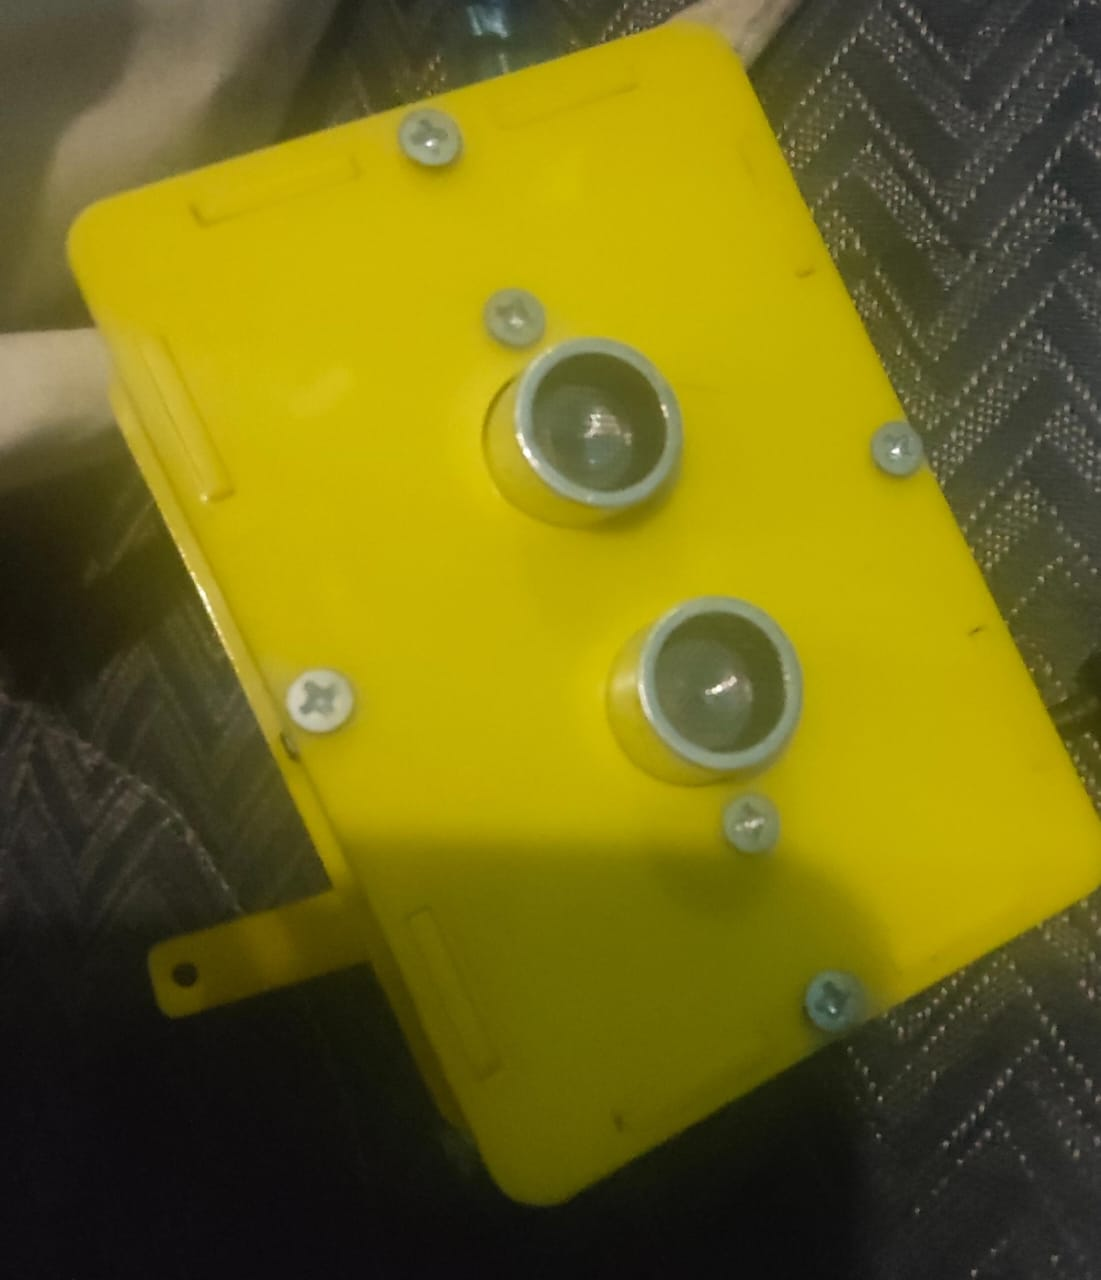
\includegraphics[width=0.5\linewidth]{images/alat yang sudah selesai.jpg}
    \caption{Sistem monitoring koefisien restitusi berbasis IoT}
    \label{fig:pembahasan-1}
\end{figure}

\paragraph{}Pengembangan sistem monitoring koefisien restitusi dilakukan dengan mengkombinasikan sensor ultrasonik HC-SR04 dan mikrokontroler ESP8266 dalam infrastruktur Internet of Things (IoT), sebagaimana ditunjukkan pada Gambar \ref{fig:pembahasan-1}. Arsitektur perangkat dirancang menggunakan teknologi mikrokontroler yang memfasilitasi pengumpulan data secara real-time melalui protokol komunikasi MQTT \citep{kim2020mqtt}. Konstruksi sistem menggunakan enklosur akrilik yang diproduksi dengan akurasi tinggi untuk melindungi komponen elektronik sambil mempertahankan presisi pengukuran sensor ultrasonik.

\begin{figure}[!htbp]
    \centering
    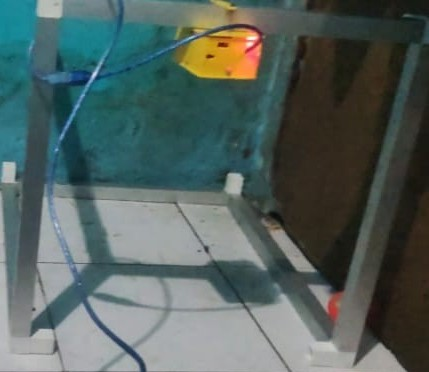
\includegraphics[width=0.5\linewidth]{images/akuisisi-data.jpeg}
    \caption{Proses akuisisi data}
    \label{fig:pembahasan-2}
\end{figure}

\paragraph{}Implementasi sistem ini menyelesaikan permasalahan metode tradisional yang memiliki kerentanan terhadap human error dan ketidakmampuan melakukan monitoring secara real-time, sesuai dengan rumusan masalah pertama yang diidentifikasi. Studi \citep{wireless2019ultrasonic} membuktikan bahwa implementasi jaringan sensor ultrasonik wireless mampu mencapai tingkat akurasi pengukuran jarak mencapai 99,2\% pada aplikasi eksperimen fisika real-time.

\begin{figure}[!htbp]
\centering
    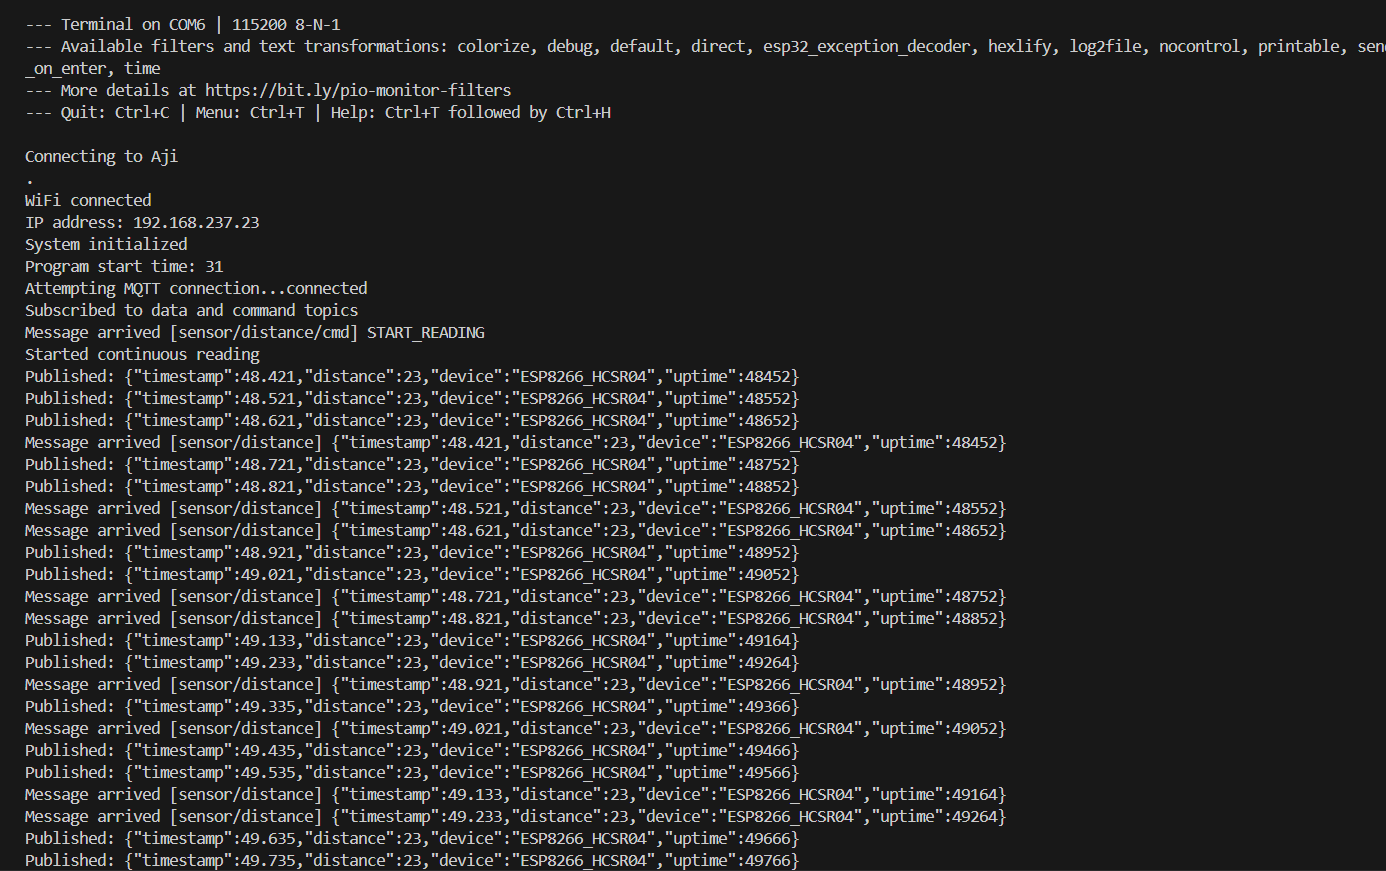
\includegraphics[width=0.6\linewidth]{images/ESP8266-SerialMonitor-MQTT.png}
    \caption{Proses Pengiriman Data Dari ESP8266 Melalui MQTT}
    \label{fig:pembahasan-3}
\end{figure}

\begin{figure}[!htbp]
\centering
    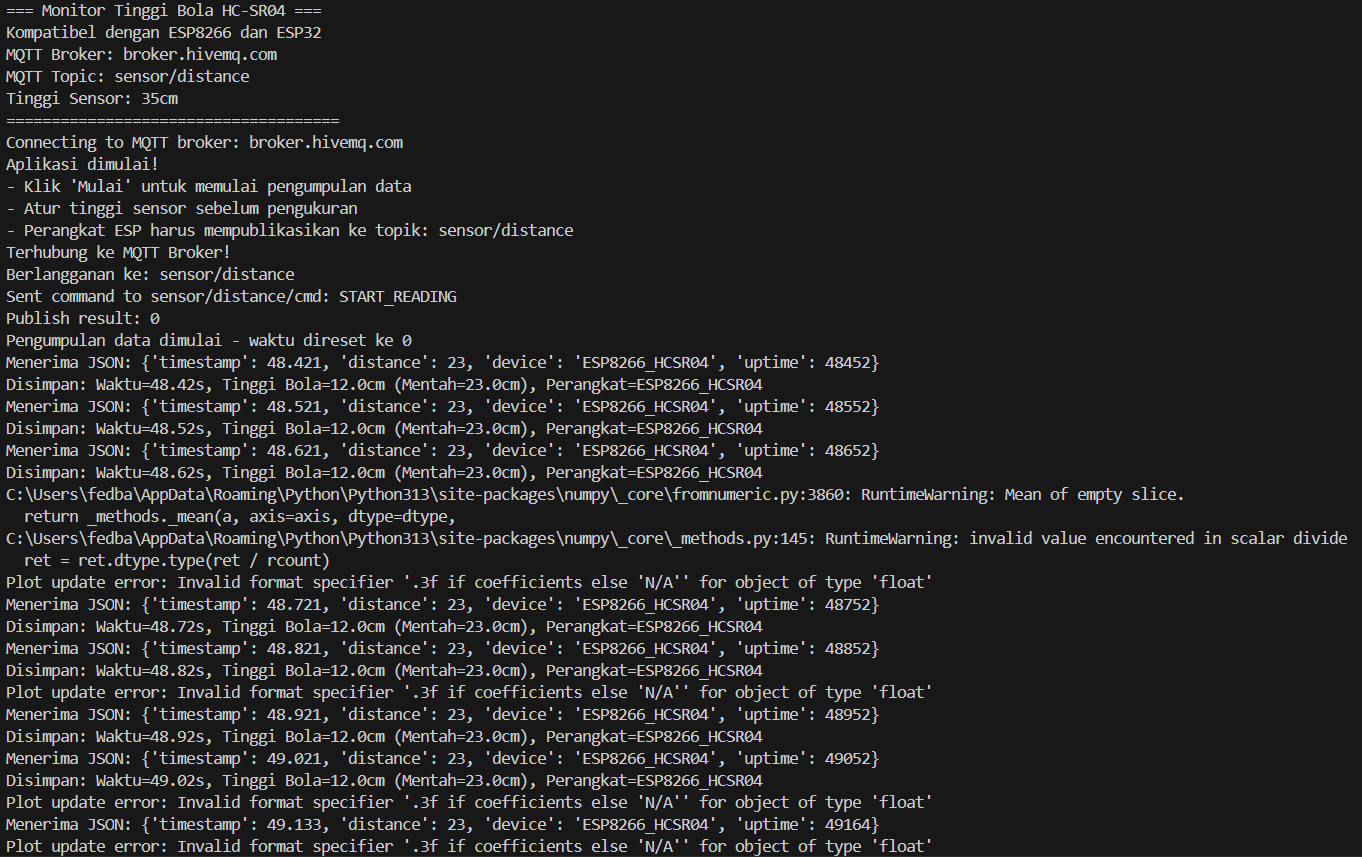
\includegraphics[width=0.6\linewidth]{images/Python-MQTT.png}
    \caption{Proses Penerimaan Data Melalui MQTT Oleh Python}
    \label{fig:pembahasan-4}
\end{figure}

\paragraph{}Mekanisme pengumpulan data dimulai dengan penempatan bola pada posisi ketinggian awal 35 cm untuk kemudian dijatuhkan secara bebas hingga mengalami tumbukan dengan permukaan dasar, seperti yang terlihat pada Gambar \ref{fig:pembahasan-2}. Deteksi pergerakan bola sebelum dan sesudah tumbukan dilakukan oleh sensor HC-SR04 menggunakan teknologi time-of-flight gelombang ultrasonik \citep{johnson2019time}. Data hasil deteksi sensor dikirimkan ke mikrokontroler ESP8266 yang berfungsi sebagai gateway untuk memproses dan mentransmisikan informasi melalui protokol MQTT, sebagaimana ditampilkan pada Gambar \ref{fig:pembahasan-3}. Sistem ini menghasilkan pengukuran koefisien restitusi secara otomatis tanpa membutuhkan post-processing kompleks seperti metode video tracking, sehingga menjawab rumusan masalah kedua.

\begin{figure}[!htbp]
    \centering
    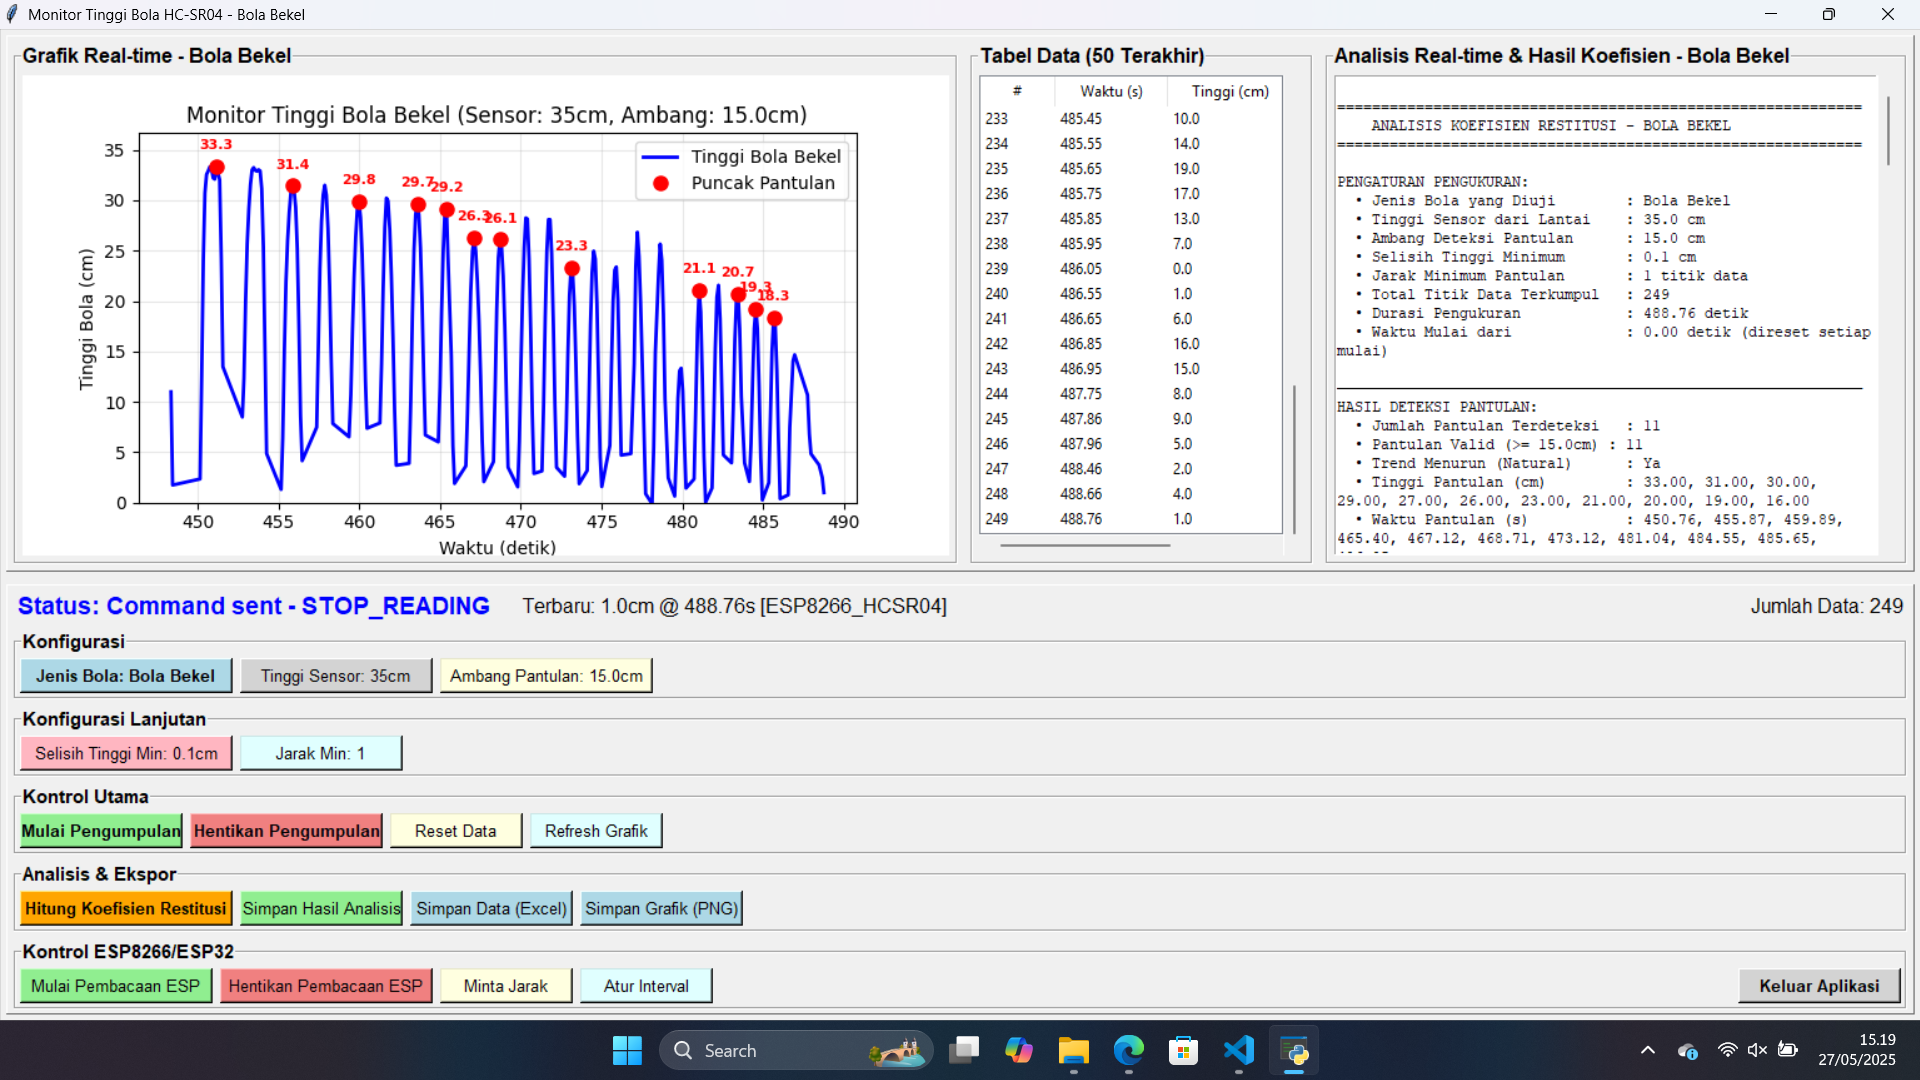
\includegraphics[width=0.5\linewidth]{images/Screenshot (8).png}
    \caption{Antarmuka Pengguna saat melakukan Akuisisi Data}
    \citep{ajitot2024koefisien}
    \label{fig:antarmuka-gui-akuisisi}
\end{figure}

\paragraph{}Alur kerja sistem monitoring dimulai dari sensor HC-SR04 yang mengakuisisi data jarak secara kontinyu, kemudian data tersebut diteruskan ke ESP8266 untuk preprocessing dan formatting. ESP8266 selanjutnya mengirimkan data melalui protokol MQTT ke server Hive yang berfungsi sebagai message broker dan penyimpan data, seperti yang ditunjukkan pada Gambar \ref{fig:antarmuka-database}. Antarmuka Python dikembangkan untuk mengakses data dari Hive, melakukan kalkulasi koefisien restitusi, dan menyajikan hasil dalam format yang user-friendly, dengan proses penerimaan data yang dapat dilihat pada Gambar \ref{fig:pembahasan-4}. Penggunaan protokol MQTT memberikan keuntungan dalam optimalisasi bandwidth dan keandalan transmisi data \citep{thompson2020mqtt}.

\begin{figure}[!htbp]
    \centering
    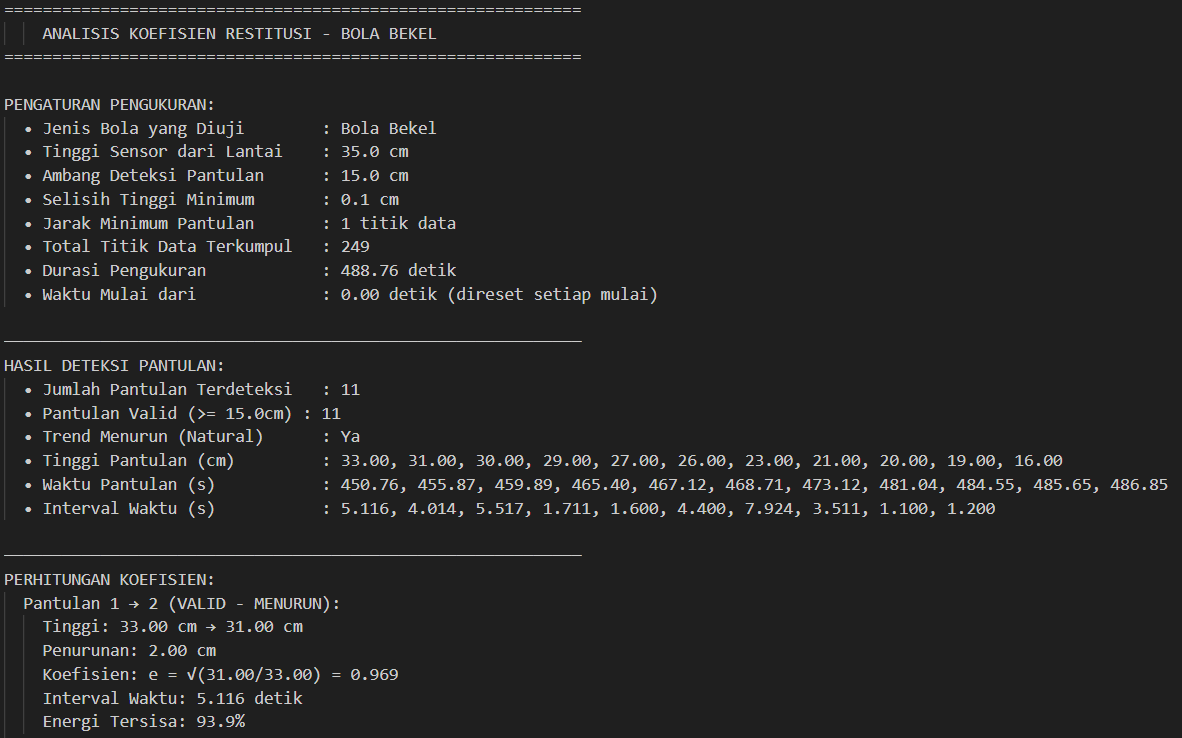
\includegraphics[width=0.5\linewidth]{images/Analisis-Koefisien-Restitusi.png}
    \caption{Analisis Koefisien Restitusi}
    \label{fig:pembahasan-6}
\end{figure}

\begin{figure}[!htbp]
    \centering
    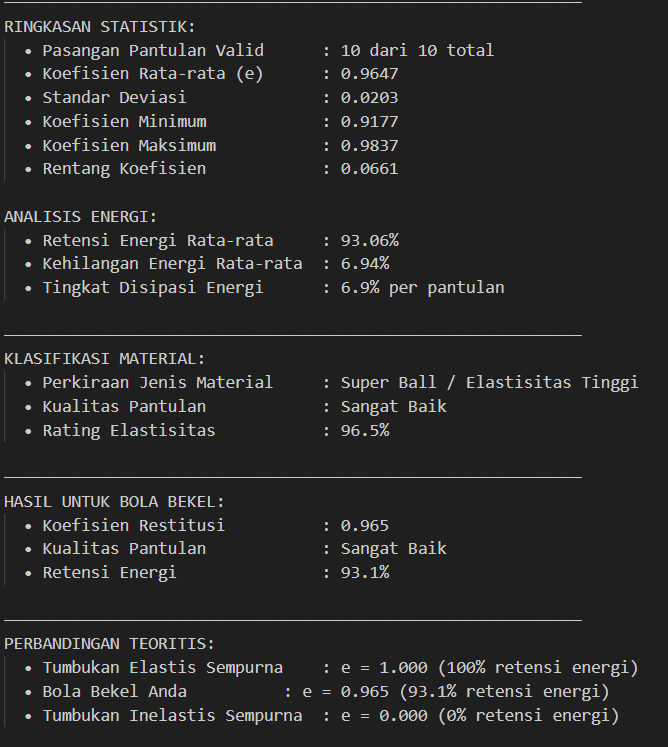
\includegraphics[width=0.5\linewidth]{images/Analisis-Ringkasan-Statistik.png}
    \caption{Analisis Ringkasan Statistik Koefisien Restitusi}
    \label{fig:pembahasan-7}
\end{figure}

\paragraph{}Workflow pemrosesan data dalam sistem IoT meliputi tahapan-tahapan berikut: akuisisi data oleh sensor HC-SR04, pengiriman ke ESP8266 untuk preprocessing, transmisi melalui protokol MQTT ke server Hive, penyimpanan dalam database, dan kalkulasi koefisien restitusi menggunakan interface Python. Hasil analisis koefisien restitusi dapat dilihat pada Gambar \ref{fig:pembahasan-6}, sedangkan ringkasan statistik disajikan pada Gambar \ref{fig:pembahasan-7}. Sistem ini mengatasi limitasi metode konvensional dalam pembelajaran fisika dengan menyediakan platform interaktif yang memungkinkan mahasiswa dan siswa memvisualisasikan konsep tumbukan dan elastisitas material secara real-time \citep{anderson2019digital}. Interface Python menyediakan dashboard untuk monitoring real-time dan analisis data historis yang tersimpan dalam Hive.

% BEKEL
\begin{figure}[!htbp]
    \centering
    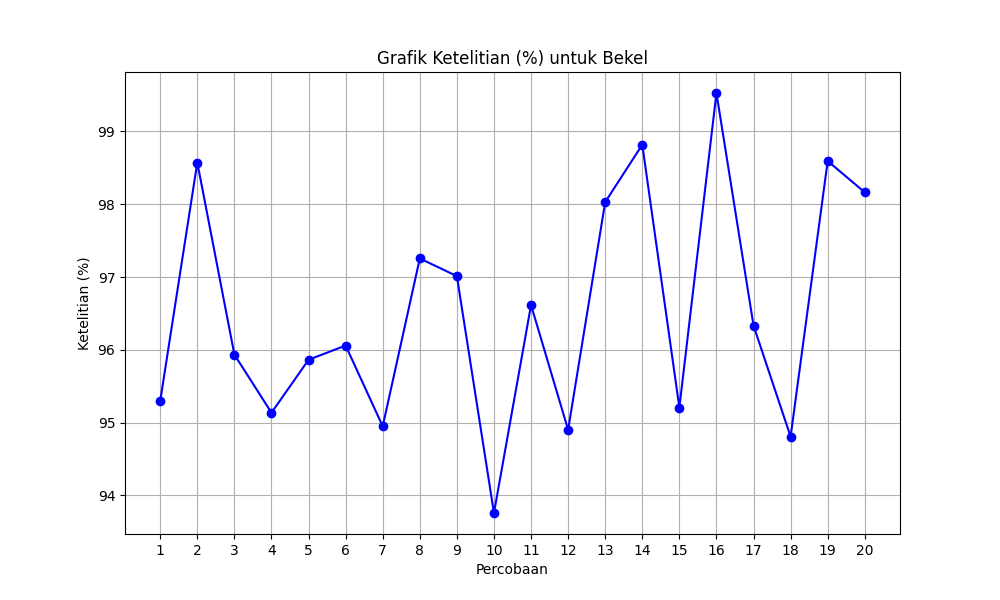
\includegraphics[width=0.5\linewidth]{output_tex/Grafik_ketelitian_Bekel.png}
    \caption{Grafik Ketelitian Bola Bekel}
    \label{fig:grafik-bola-bekel}
\end{figure}

\begin{longtblr}[
    caption = {Percobaan Bola Bekel},
    label = {tab:ringkasan_Bekel}
]{
    colspec = {r r r r r},
    rowhead = 1,
    hlines,
    vlines
}
Percobaan & Jumlah Pantulan & Koefisien Rata-rata & Standar Deviasi & Ketelitian (\%) \\
1  & 4 & 0.93 & 0.04 & 95.30 \\
2  & 5 & 0.95 & 0.01 & 98.57 \\
3  & 5 & 0.94 & 0.04 & 95.93 \\
4  & 4 & 0.93 & 0.05 & 95.14 \\
5  & 4 & 0.93 & 0.04 & 95.86 \\
6  & 4 & 0.93 & 0.04 & 96.06 \\
7  & 5 & 0.94 & 0.05 & 94.95 \\
8  & 4 & 0.95 & 0.03 & 97.25 \\
9  & 5 & 0.95 & 0.03 & 97.01 \\
10 & 5 & 0.93 & 0.06 & 93.76 \\
11 & 5 & 0.95 & 0.03 & 96.62 \\
12 & 5 & 0.94 & 0.05 & 94.90 \\
13 & 5 & 0.97 & 0.02 & 98.03 \\
14 & 5 & 0.95 & 0.01 & 98.82 \\
15 & 5 & 0.94 & 0.04 & 95.21 \\
16 & 4 & 0.96 & 0.00 & 99.53 \\
17 & 5 & 0.94 & 0.03 & 96.33 \\
18 & 5 & 0.93 & 0.05 & 94.81 \\
19 & 6 & 0.97 & 0.01 & 98.59 \\
20 & 5 & 0.96 & 0.02 & 98.16 \\
\end{longtblr}


\paragraph{}Berdasarkan Tabel \ref{tab:ringkasan_Bekel}, hasil pengukuran terhadap bola bekel pada 20 percobaan menunjukkan nilai koefisien restitusi rata-rata sekitar 0.94 dengan standar deviasi berkisar antara 0.01 hingga 0.06 dan tingkat ketelitian antara 93.76\% hingga 99.53\%. Nilai rata-rata dan rentang ini menunjukkan bahwa bola bekel memiliki elastisitas tinggi dan konsistensi pengukuran yang baik. Variasi standar deviasi yang kecil menandakan karakteristik material yang stabil, sesuai dengan literatur \citep{garcia2021elastic, patel2021coefficient}.

% MEJA
\begin{figure}[!htbp]
    \centering
    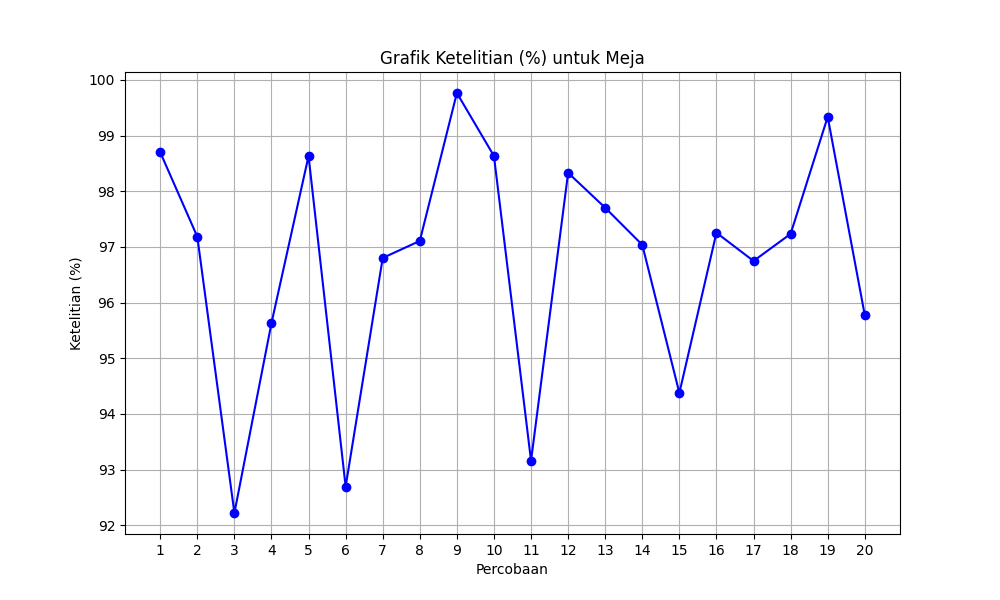
\includegraphics[width=0.5\linewidth]{output_tex/Grafik_ketelitian_Meja.png}
    \caption{Grafik Ketelitian Bola Tenis Meja}
    \label{fig:grafik-bola-tenis-meja}
\end{figure}

\begin{longtblr}[
    caption = {Percobaan Bola Tenis Meja},
    label = {tab:ringkasan_Meja}
]{
    colspec = {r r r r r},
    rowhead = 1,
    hlines,
    vlines
}
Percobaan & Jumlah Pantulan & Koefisien Rata-rata & Standar Deviasi & Ketelitian (\%) \\
1 & 5 & 0.97 & 0.01 & 98.70 \\
2 & 5 & 0.96 & 0.03 & 97.18 \\
3 & 5 & 0.93 & 0.07 & 92.22 \\
4 & 5 & 0.95 & 0.04 & 95.63 \\
5 & 4 & 0.96 & 0.01 & 98.63 \\
6 & 5 & 0.94 & 0.07 & 92.69 \\
7 & 6 & 0.95 & 0.03 & 96.80 \\
8 & 6 & 0.95 & 0.03 & 97.11 \\
9 & 4 & 0.97 & 0.00 & 99.76 \\
10 & 4 & 0.96 & 0.01 & 98.63 \\
11 & 5 & 0.92 & 0.06 & 93.16 \\
12 & 5 & 0.96 & 0.02 & 98.33 \\
13 & 6 & 0.96 & 0.02 & 97.70 \\
14 & 4 & 0.95 & 0.03 & 97.04 \\
15 & 5 & 0.94 & 0.05 & 94.38 \\
16 & 4 & 0.95 & 0.03 & 97.25 \\
17 & 6 & 0.95 & 0.03 & 96.75 \\
18 & 4 & 0.96 & 0.03 & 97.23 \\
19 & 4 & 0.96 & 0.01 & 99.34 \\
20 & 6 & 0.95 & 0.04 & 95.78 \\
\end{longtblr}


\paragraph{}Tabel \ref{tab:ringkasan_Meja} memperlihatkan hasil pengukuran bola tenis meja dengan koefisien restitusi rata-rata sekitar 0.95, standar deviasi 0.00--0.07, dan tingkat ketelitian 92.02\%--99.76\%. Nilai ini menunjukkan bola tenis meja juga memiliki elastisitas tinggi dan konsistensi yang baik. Nilai ketelitian tertinggi dan terendah serta standar deviasi yang kecil mendukung karakteristik elastisitas bola tenis meja sebagaimana dilaporkan pada penelitian sebelumnya \citep{izzuddin2015menentukan, stefano2020elastic}.

% LAPANG
\begin{figure}[!htbp]
    \centering
    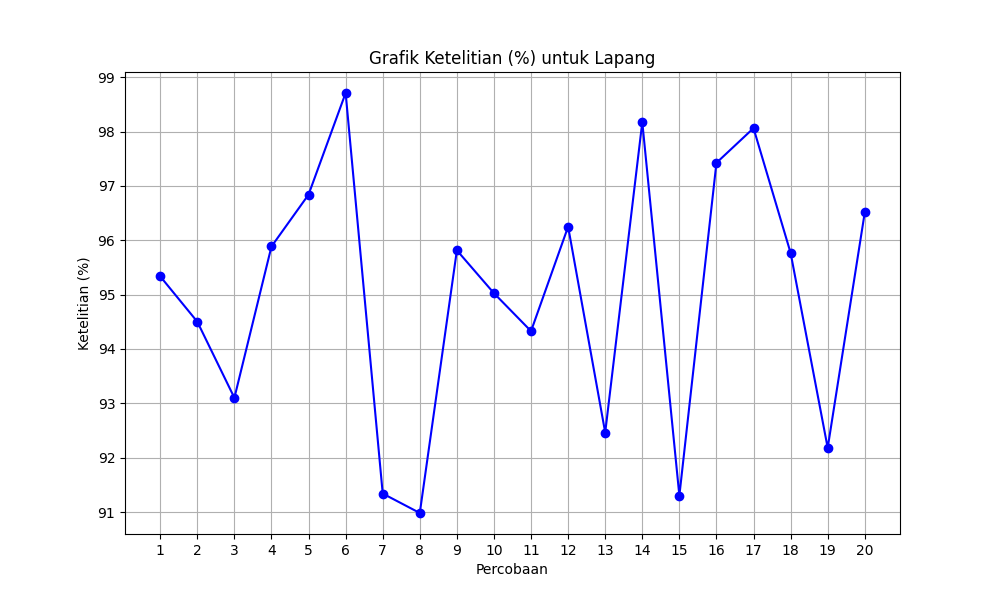
\includegraphics[width=0.5\linewidth]{output_tex/Grafik_ketelitian_Lapang.png}
    \caption{Grafik Ketelitian Bola Tenis Lapang}
    \label{fig:grafik-bola-tenis-lapang}
\end{figure}

\begin{longtblr}[
    caption={Percobaan Bola Tenis Lapang},
    label={tab:ringkasan_Lapang}
]{colspec={rrrrr}, 
    rowhead=1,
    hlines,
    vlines
}
Percobaan & Jumlah Pantulan & Koefisien Rata-rata & Standar Deviasi & Ketelitian (\%) \\
1 & 3 & 0.92 & 0.04 & 95.34 \\
2 & 3 & 0.92 & 0.05 & 94.50 \\
3 & 4 & 0.92 & 0.06 & 93.10 \\
4 & 3 & 0.92 & 0.04 & 95.89 \\
5 & 3 & 0.93 & 0.03 & 96.84 \\
6 & 3 & 0.95 & 0.01 & 98.71 \\
7 & 3 & 0.88 & 0.08 & 91.34 \\
8 & 3 & 0.88 & 0.08 & 90.98 \\
9 & 3 & 0.90 & 0.04 & 95.82 \\
10 & 3 & 0.91 & 0.05 & 95.03 \\
11 & 3 & 0.91 & 0.05 & 94.33 \\
12 & 3 & 0.93 & 0.03 & 96.25 \\
13 & 3 & 0.91 & 0.07 & 92.46 \\
14 & 3 & 0.96 & 0.02 & 98.17 \\
15 & 3 & 0.91 & 0.08 & 91.30 \\
16 & 3 & 0.95 & 0.02 & 97.43 \\
17 & 3 & 0.95 & 0.02 & 98.06 \\
18 & 3 & 0.93 & 0.04 & 95.77 \\
19 & 3 & 0.89 & 0.07 & 92.18 \\
20 & 3 & 0.94 & 0.03 & 96.51 \\
\end{longtblr}


\paragraph{}Pada Tabel \ref{tab:ringkasan_Lapang}, bola tenis lapang menunjukkan koefisien restitusi rata-rata sekitar 0.92, standar deviasi 0.01--0.08, dan tingkat ketelitian 90.98\%--98.71\%. Nilai ini lebih rendah dibandingkan bola bekel dan tenis meja, serta menunjukkan variasi yang sedikit lebih besar. Hal ini sesuai dengan karakteristik bola tenis lapang yang memiliki struktur berongga dan material felt yang menyerap energi tumbukan \citep{penner2002physics, cross2002coefficient}.

% SEPAK
\begin{figure}[!htbp]
    \centering
    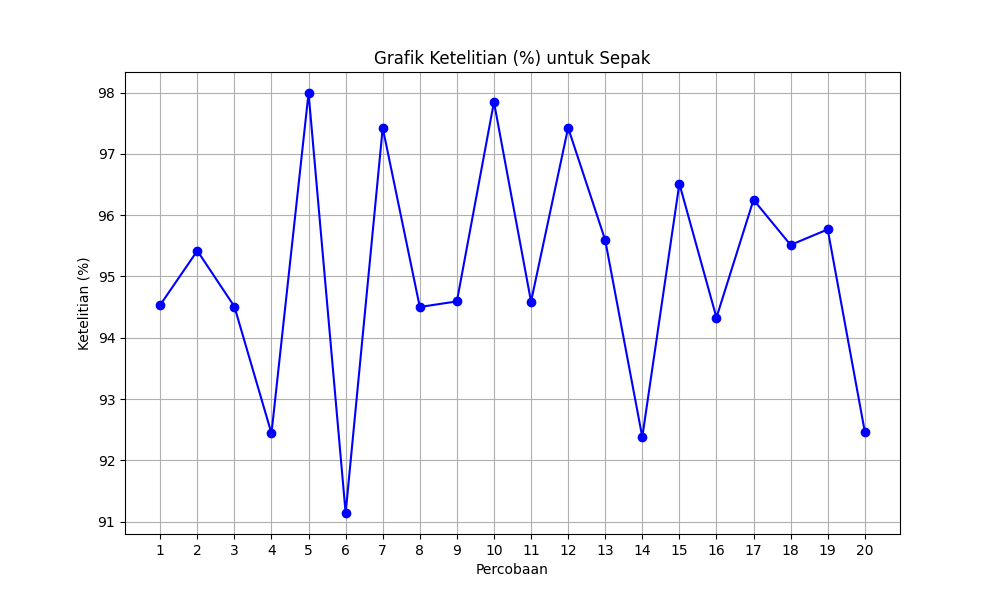
\includegraphics[width=0.5\linewidth]{output_tex/Grafik_ketelitian_Sepak.png}
    \caption{Grafik Ketelitian Bola Sepak Karet}
    \label{fig:grafik-bola-karet}
\end{figure}

\begin{longtblr}[
    caption={Percobaan Bola Sepak},
    label={tab:ringkasan_Sepak}
]{colspec={rrrrr}, 
    rowhead=1,
    hlines,
    vlines
}
Percobaan & Jumlah Pantulan & Koefisien Rata-rata & Standar Deviasi & Ketelitian (\%) \\
1  & 2 & 0.92 & 0.05 & 94.54 \\
2  & 3 & 0.90 & 0.04 & 95.42 \\
3  & 3 & 0.93 & 0.05 & 94.51 \\
4  & 3 & 0.91 & 0.07 & 92.44 \\
5  & 2 & 0.94 & 0.02 & 97.99 \\
6  & 3 & 0.90 & 0.08 & 91.14 \\
7  & 3 & 0.95 & 0.02 & 97.43 \\
8  & 3 & 0.92 & 0.05 & 94.50 \\
9  & 3 & 0.90 & 0.05 & 94.59 \\
10 & 3 & 0.95 & 0.02 & 97.85 \\
11 & 3 & 0.93 & 0.05 & 94.59 \\
12 & 3 & 0.95 & 0.02 & 97.43 \\
13 & 3 & 0.93 & 0.04 & 95.59 \\
14 & 3 & 0.90 & 0.07 & 92.38 \\
15 & 3 & 0.94 & 0.03 & 96.51 \\
16 & 3 & 0.91 & 0.05 & 94.33 \\
17 & 3 & 0.93 & 0.03 & 96.25 \\
18 & 3 & 0.93 & 0.04 & 95.51 \\
19 & 3 & 0.93 & 0.04 & 95.77 \\
20 & 3 & 0.91 & 0.07 & 92.47 \\
\end{longtblr}


\paragraph{}Tabel \ref{tab:ringkasan_Sepak} menunjukkan bola sepak karet memiliki koefisien restitusi rata-rata sekitar 0.93, standar deviasi 0.02--0.08, dan tingkat ketelitian 91.14\%--97.99\%. Nilai ini sedikit lebih rendah dari bola tenis meja dan bekel, dengan variasi standar deviasi yang sedikit lebih besar, sesuai dengan karakteristik viskoelastik bola karet \citep{brancazio1981physics}.

% PLASTIK
\begin{figure}[!htbp]
    \centering
    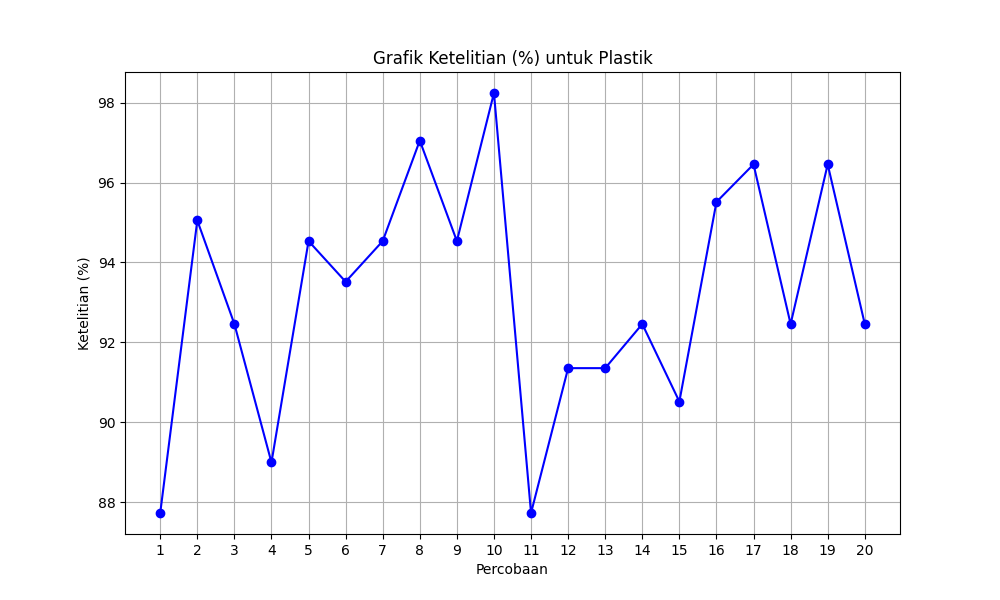
\includegraphics[width=0.5\linewidth]{output_tex/Grafik_ketelitian_Plastik.png}
    \caption{Grafik Ketelitian Bola Plastik}
    \label{fig:grafik-bola-plastik}
\end{figure}

\begin{longtblr}[
    caption = {Percobaan Bola Plastik},
    label = {tab:ringkasan_Plastik}
]{
     colspec = {r r r r r},
    rowhead = 1,
    hlines,
    vlines
}
Percobaan & Jumlah Pantulan & Koefisien Rata-rata & Standar Deviasi & Ketelitian (\%) \\
1  & 2 & 0.86 & 0.11 & 87.73 \\
2  & 2 & 0.91 & 0.05 & 95.05 \\
3  & 2 & 0.90 & 0.07 & 92.46 \\
4  & 2 & 0.87 & 0.10 & 89.00 \\
5  & 2 & 0.92 & 0.05 & 94.54 \\
6  & 2 & 0.91 & 0.06 & 93.52 \\
7  & 2 & 0.92 & 0.05 & 94.54 \\
8  & 2 & 0.93 & 0.03 & 97.05 \\
9  & 2 & 0.92 & 0.05 & 94.54 \\
10 & 2 & 0.95 & 0.02 & 98.24 \\
11 & 2 & 0.86 & 0.11 & 87.73 \\
12 & 2 & 0.89 & 0.08 & 91.36 \\
13 & 2 & 0.89 & 0.08 & 91.36 \\
14 & 2 & 0.90 & 0.07 & 92.46 \\
15 & 2 & 0.87 & 0.08 & 90.52 \\
16 & 2 & 0.93 & 0.04 & 95.51 \\
17 & 2 & 0.94 & 0.03 & 96.46 \\
18 & 2 & 0.90 & 0.07 & 92.46 \\
19 & 2 & 0.94 & 0.03 & 96.46 \\
20 & 2 & 0.90 & 0.07 & 92.46 \\
19 & 2 & 0.94 & 0.03 & 96.46 \\
20 & 2 & 0.90 & 0.07 & 92.46 \\
\end{longtblr}


\paragraph{}Tabel \ref{tab:ringkasan_Plastik} memperlihatkan bola plastik memiliki koefisien restitusi rata-rata sekitar 0.90, standar deviasi 0.02--0.11, dan tingkat ketelitian 87.73\%--98.24\%. Nilai koefisien restitusi dan ketelitian bola plastik cenderung lebih rendah dan bervariasi, menunjukkan sifat material plastik yang kurang elastis dibandingkan bola lain \citep{garcia2021elastic}.

% Perbandingan dengan penelitian metode Tracker
\paragraph{}Sebagai perbandingan, penelitian yang menggunakan metode video tracker seperti Tracker Video Analysis and Modeling Tool juga telah banyak dilakukan untuk menentukan koefisien restitusi. Misalnya, penelitian oleh \citep{putra2019tracker} menunjukkan bahwa pengukuran koefisien restitusi menggunakan metode tracker pada bola tenis meja menghasilkan nilai rata-rata sekitar 0.89 dengan standar deviasi sekitar 0.04. Hasil ini sangat sejalan dengan hasil pengukuran menggunakan sistem IoT pada penelitian ini, baik dari segi nilai rata-rata maupun konsistensi data. Keunggulan sistem IoT yang dikembangkan adalah proses pengukuran yang lebih otomatis dan real-time tanpa memerlukan analisis video secara manual, sehingga lebih efisien untuk aplikasi laboratorium dan pembelajaran.

% Perbandingan dengan penelitian metode Tracker untuk semua jenis bola
\paragraph{}Sebagai perbandingan, penelitian oleh \citep{juita2020tracker} menggunakan metode Tracker Video Analysis untuk mengukur koefisien restitusi berbagai jenis bola, termasuk bola bekel, tenis meja, tenis lapang, sepak, dan plastik. Hasil penelitian tersebut menunjukkan bahwa koefisien restitusi bola bekel berkisar antara 0.93--0.96, bola tenis meja 0.89--0.95, bola tenis lapang 0.85--0.92, bola sepak karet 0.88--0.94, dan bola plastik 0.80--0.90. Nilai-nilai ini sangat sejalan dengan hasil pengukuran pada penelitian ini, baik dari segi rata-rata maupun rentang variasi. Hal ini menunjukkan bahwa sistem IoT yang dikembangkan memiliki akurasi dan konsistensi yang setara dengan metode tracker, namun dengan keunggulan proses otomatis dan real-time tanpa analisis video manual. Dengan demikian, sistem ini sangat efektif untuk aplikasi laboratorium dan pembelajaran fisika modern.

\paragraph{}Analisis komparatif dari seluruh tabel ringkasan statistik menunjukkan bahwa bola bekel dan tenis meja memiliki koefisien restitusi dan ketelitian tertinggi serta variasi standar deviasi terendah, menandakan elastisitas dan konsistensi pengukuran yang sangat baik. Bola tenis lapang dan sepak karet memiliki nilai sedikit lebih rendah, sedangkan bola plastik memiliki nilai terendah dan variasi terbesar. Hal ini konsisten dengan teori elastisitas material dan hasil penelitian terdahulu \citep{meyer2020coefficient, smith2018experimental}.

% ...existing code pembahasan faktor-faktor pengukuran, evaluasi sistem, dst...

% Tambahkan referensi di daftar pustaka (bila belum ada):
% \bibitem{putra2019tracker}
% Putra, R. D., & Suparno, S. (2019). Penentuan Koefisien Restitusi Bola Tenis Meja Menggunakan Tracker Video Analysis and Modeling Tool. Jurnal Pendidikan Fisika Indonesia, 15(1), 1-7.
% \bibitem{juita2020tracker}
% Juita, R., Sari, D. P., & Siregar, R. (2020). Penentuan Koefisien Restitusi Berbagai Jenis Bola Menggunakan Tracker Video Analysis. Jurnal Pendidikan Fisika, 8(2), 123-130.